\documentclass[11pt,letterpaper]{article}

\usepackage[margin=1in]{geometry}
\usepackage{amsmath,amssymb,amsthm}
\usepackage{booktabs}
\usepackage{graphicx}
\usepackage{xcolor}
\usepackage{enumitem}
\usepackage{microtype}
\usepackage{tcolorbox}
\tcbuselibrary{skins,breakable}
\usepackage[colorlinks=true,linkcolor=blue!70!black,citecolor=blue!70!black,urlcolor=blue!70!black]{hyperref}

% Style definitions
\theoremstyle{definition}
\newtheorem{definition}{Definition}[section]
\newtheorem{example}{Example}[section]
\theoremstyle{plain}
\newtheorem{theorem}{Theorem}[section]
\newtheorem{lemma}[theorem]{Lemma}
\newtheorem{proposition}[theorem]{Proposition}
\newtheorem{corollary}[theorem]{Corollary}
\theoremstyle{remark}
\newtheorem{remark}{Remark}[section]

% Colored boxes for key insights and definitions
\newtcolorbox{takeawaybox}[1][]{
  colback=blue!5!white,
  colframe=blue!65!black,
  fonttitle=\bfseries,
  title=#1,
  arc=3mm,
  breakable,
  boxrule=0.8pt
}

\newtcolorbox{warningbox}[1][]{
  colback=red!5!white,
  colframe=red!65!black,
  fonttitle=\bfseries,
  title=#1,
  arc=3mm,
  breakable,
  boxrule=0.8pt
}

\newtcolorbox{ideabox}[1][]{
  colback=green!5!white,
  colframe=green!50!black,
  fonttitle=\bfseries,
  title=#1,
  arc=3mm,
  breakable,
  boxrule=0.8pt
}

\title{\textbf{\LARGE Two-Sided Matching on Modern Dating Platforms}\\[0.4em]
\Large From Match Counting to Per-Person Quality and Incentive-Compatible Mechanism Design\\[0.8em]
\large A Comprehensive Research Monograph and Project Guide}
\author{\textbf{CS 580: Algorithmic Game Theory Project}\\[0.2em]
Collaborative Research Synthesis}
\date{October 2026}

\begin{document}

\maketitle

\begin{abstract}
Online dating platforms mediate romantic search for hundreds of millions of users by deciding which profile assortments to display over time. Historically, algorithmic market design in this space focused either on static, centralized clearinghouses (e.g., Gale-Shapley Deferred Acceptance) or dynamic optimization aimed strictly at maximizing the \emph{expected raw number of matches} (such as the recent Integral Dating Heuristic of Rios \& Torrico, 2026). However, real users do not value ten mediocre matches more than one compatible partner; they care about \emph{match quality}, and ultimately their \emph{single best match}. Furthermore, users interact with platforms strategically rather than mechanically.

This monograph provides a completely self-contained, rigorous, and accessible exposition of this problem space. We detail: (1) the foundational Rios \& Torrico (2026) dynamic assortment framework and its core mathematical mechanism; (2) our audit and machine-checked repair of the published multi-period heuristics; (3) the transition from match count to additive match quality, which sharpens the classical $1-1/e$ bound to the exact uniform-matroid correlation gap $c_K = 1 - e^{-K}K^K/K!$; (4) the transition to per-person top-$k$ match quality, showing why standard methods lose over 50\% of welfare and how our new \emph{Credit-DH} algorithm restores provable constant-factor guarantees; (5) the game-theoretic layer of strategic users, clarifying the vital distinction between platform capacity constraints and user reservation costs; (6) our \emph{Screened Dating Heuristic (SDH)}, which leverages LLM evaluation oracles to guarantee that truthful, sincere swiping is a Dominant Strategy (DSIC); and (7) a critical analysis of where these mathematical assumptions break down in production applications like Tinder, Bumble, and Hinge.
\end{abstract}

\vspace{1em}
\tableofcontents
\newpage

% =============================================================================
\section{Introduction and Foundational Motivation}
\label{sec:intro}
% =============================================================================

Matching markets have occupied a central place in algorithmic game theory and economic design since the seminal work of Gale and Shapley (1962). While early market design focused on centralized clearinghouses—such as medical residency matching, school choice, and kidney exchange—the explosive rise of online dating applications (Tinder, Bumble, Hinge, Coffee Meets Bagel) presents a radically different paradigm:
\begin{itemize}[leftmargin=2em]
    \item \textbf{Decentralized, sequential interaction}: Agents do not submit an exhaustive preference list to an omniscient central coordinator. Instead, search unfolds dynamically over discrete time periods.
    \item \textbf{Strict attention and capacity limits}: In any period, each user can be shown only a small display of $K$ candidate profiles.
    \item \textbf{Asymmetric, asynchronous interest}: Matches require mutual consent, but likes are realized sequentially across time. A pending like sits in a user's ``backlog'' until the platform decides to surface it.
    \item \textbf{Computational intractability}: The exact dynamic program that tracks all possible combinations of past likes, pending backlogs, and future arrivals across thousands of interacting agents suffers from a combinatorial state space that grows exponentially with the horizon $T$.
\end{itemize}

\subsection{The Quality vs. Quantity Paradox}
In their foundational 2026 paper, \emph{``The Dating Heuristic: A Provably Strong Matching Algorithm for Dating Platforms,''} Ignacio Rios and Alfredo Torrico formulated an elegant, tractable mixed-integer program lookahead (\textbf{DH-int}) that balances immediate display decisions against future backlog reciprocations, proving a $(1 - 1/e) \approx 0.632$ approximation against the optimal adaptive dynamic program.

However, the objective of the Rios \& Torrico paper is almost exclusively the \textbf{expected total count of matches}:
\begin{equation}
    \max \quad \mathbb{E} \left[ |\mathcal{M}| \right] = \mathbb{E}\left[ \sum_{t=1}^T \sum_{(i,j)} \mu_{ij}^t \right].
\end{equation}
While maximizing raw match count is a natural starting point for revenue models centered on user activity, it produces severe market distortions:
\begin{enumerate}[leftmargin=2em]
    \item \textbf{The Dilution Problem}: Ten low-compatibility matches are treated by the objective as ten times more valuable than a single life partner.
    \item \textbf{Congestion and Swamping}: Unweighted algorithms routinely herd attention toward candidates with high marginal like probabilities, even if their ultimate mutual compatibility is near zero.
    \item \textbf{The Best-Match Breakdown}: Ultimately, a user seeking a monogamous relationship is searching for their \emph{single best match} ($k=1$). A policy that gives a user five mediocre matches and zero great matches is treated as superior to a policy that gives that user one soulmate.
\end{enumerate}

\subsection{The Roadmap of this Monograph}
This project has systematically expanded the dating heuristic framework along three distinct frontiers:
\begin{enumerate}[leftmargin=2em]
    \item \textbf{Theoretical Audit \& Repair}: Formalizing the paper's multi-period proofs in Lean 4 revealed that the multi-period theorems (Theorems 5.3 and 5.4 in Rios \& Torrico) are false as published due to timing pooling flaws. We present our machine-checked counterexamples and the time-indexed repaired algorithm, \textbf{DHT-$\tau$}.
    \item \textbf{From Count to Quality (Additive and Top-$k$)}: We introduce cardinal match quality $q_{\ell\ell'}$. We show that additive quality preserves approximation guarantees while sharpening the constant from $1-1/e \approx 0.632$ to $c_K = 1 - e^{-K}K^K/K!$ (e.g., $c_3 \approx 0.776$). We then reveal why top-$1$ quality breaks all standard additive LP lookaheads, and how our new \textbf{Credit-DH} algorithm solves this via contention resolution.
    \item \textbf{The Game-Theoretic Frontier (Strategic Swiping)}: When users are strategic, swiping behavior is endogenous. We clarify the difference between platform capacity constraints and user reservation costs, characterize the exact conditions under which truthful swiping is a dominant strategy (\textbf{Cost-Separability}), and present our \textbf{Screened Dating Heuristic (SDH)} with an LLM oracle.
\end{enumerate}

\begin{takeawaybox}[Clarifying the Terminology: ``Costs'' vs. ``Budgets'' vs. ``Quality'']
Throughout this monograph, three distinct concepts govern the interaction:
\begin{itemize}[leftmargin=1.5em]
    \item \textbf{Compatibility Quality ($q_{\ell\ell'} \ge 0$)}: The cardinal happiness or romantic value that user $\ell$ derives from being matched with profile $\ell'$.
    \item \textbf{Platform Capacity / Display Budget ($K_\ell$)}: The physical limit on how many profiles user $\ell$ is allowed to see (or swipe on) in each period. In the platform's optimization, displaying a candidate ``costs'' 1 unit of this display quota.
    \item \textbf{User Reservation / Match Cost ($c_\ell \ge 0$)}: In the game-theoretic setting, a match is not free to the user—it requires time, chatting effort, and going on dates. A user only experiences positive surplus if $q_{\ell\ell'} > c_\ell$. If $c_\ell = 0$, swiping is costless, meaning users have no reason to ever swipe left!
\end{itemize}
\end{takeawaybox}

\newpage
% =============================================================================
\section{The Foundational Paper: Rios \& Torrico (2026)}
\label{sec:paper}
% =============================================================================

\subsection{The Mathematical Market Model}
Consider a two-sided platform operating over a finite discrete horizon $t \in \{1, 2, \dots, T\}$. The market consists of two fixed disjoint sets of users, $I$ (e.g., men) and $J$ (e.g., women). Let $U = I \cup J$.

\begin{itemize}[leftmargin=2em]
    \item \textbf{Display Assortments and Capacities}: In each period $t$, the platform selects an assortment of profiles $S_\ell^t$ to display to user $\ell$. The assortment size cannot exceed the user's per-period display cap:
    \begin{equation}
        |S_\ell^t| \le K_\ell, \quad \forall \ell \in U, \; \forall t \in [T].
    \end{equation}
    \item \textbf{Potentials}: User $\ell$ can only be shown candidates from their initial feasible set $\mathcal{P}_\ell^1$ (profiles satisfying basic age, distance, and stated criteria). Once a profile is shown or a user expresses disinterest, they are removed from future consideration.
    \item \textbf{Like Probabilities and No Substitution}: When user $\ell$ is shown profile $\ell'$ in period $t$, $\ell$ likes $\ell'$ with probability $\phi_{\ell\ell'}^t$. A foundational modeling assumption of the paper is that \textbf{likes are independent across profiles shown together in the same assortment}. That is, seeing profile A does not diminish the likelihood of liking profile B in the same period.
    \item \textbf{The Backlog ($\mathcal{B}_\ell^t$)}: The backlog contains all potential partners who have already been shown profile $\ell$ in an earlier period and swiped right on $\ell$, but who have not yet been displayed to $\ell$.
\end{itemize}

\subsection{Two Mechanisms of Match Formation}
A match forms if and only if two users mutually like each other. In this dynamic setting, matches happen in one of two ways:
\begin{enumerate}[leftmargin=2em]
    \item \textbf{Sequential Matches (via Backlog)}:
    \begin{itemize}
        \item In period $t_1$, user $i$ is shown profile $j$ as an \emph{initiation}. User $i$ likes $j$ (probability $\phi_{ij}^{t_1}$).
        \item User $i$ enters $j$'s backlog $\mathcal{B}_j^{t_1+1}$.
        \item In period $t_2 > t_1$, the platform shows $i$ to $j$ from $j$'s backlog.
        \item User $j$ likes $i$ back (probability $\phi_{ji}^{t_2}$). A sequential match is formed!
    \end{itemize}
    \item \textbf{Non-Sequential (Mutual View) Matches}:
    \begin{itemize}
        \item Both users $i$ and $j$ are shown to each other in the exact same period $t$.
        \item A match forms if both like each other simultaneously, which occurs with probability $\beta_e^t = \phi_{ij}^t \phi_{ji}^t$.
    \end{itemize}
\end{enumerate}

\subsection{Decision Variables and Platform Designs}
To formalize the optimization problem, let $E = I \times J$ denote potential edges. In each period $t$:
\begin{itemize}[leftmargin=2em]
    \item $x_{\ell\ell'}^t \in \{0, 1\}$: The platform displays profile $\ell'$ to user $\ell$ along directed arc $\ell \to \ell'$. This can represent an initiation or a backlog response.
    \item $w_e^t \in \{0, 1\}$: The platform selects pair $e = \{i, j\}$ for a mutual view in period $t$.
\end{itemize}
Each pair can be displayed at most once and in at most one direction over the horizon:
\begin{equation}
    \sum_{t=1}^T \left( x_{ij}^t + x_{ji}^t + w_e^t \right) \le 1, \quad \forall e = \{i,j\}.
\end{equation}

The platform structure dictates the allowable design $\Pi$:
\begin{itemize}[leftmargin=2em]
    \item \textbf{One-directional}: Only one side (e.g., $I$) initiates. The other side ($J$) is only ever shown users from their backlog (e.g., Coffee Meets Bagel's ``Ladies Choice'').
    \item \textbf{Two-directional}: Either side can initiate, but pairs cannot be initiated simultaneously.
    \item \textbf{Sequential-only}: Mutual views are forbidden ($w_e^t = 0$ for all $t$).
\end{itemize}

\subsection{The Two-Period Model and the Integral Dating Heuristic (DH-int)}
To overcome the curse of dimensionality of the $T$-period dynamic program, Rios \& Torrico focus heavily on a two-period lookahead framework. In period 1, the backlog is empty. In period 2, all remaining actions are backlog responses (no mutual views in period 2, $w_e^2 = 0$).

The platform solves the following Mixed-Integer Program (\textbf{DH-int}, formulation 16 in the paper):
\begin{align}
    \max_{x^1, w^1, x^2} \quad & \sum_{e \in E} \beta_e w_e^1 + \sum_{\ell \in U} \sum_{\ell' \in \mathcal{P}_\ell} \phi_{\ell\ell'}^2 x_{\ell\ell'}^2 \label{eq:dh_obj} \\
    \text{subject to} \quad & \sum_{\ell'} x_{\ell\ell'}^1 + \sum_{e \ni \ell} w_e^1 \le K_\ell, \quad \forall \ell \in U \tag{P1: Period 1 Capacity} \\
    & x_{\ell\ell'}^1 + x_{\ell'\ell}^1 + w_e^1 \le 1, \quad \forall e = \{\ell, \ell'\} \tag{P2: Single Exposure} \\
    & 0 \le x_{\ell\ell'}^2 \le \phi_{\ell'\ell}^1 x_{\ell'\ell}^1, \quad \forall \ell, \ell' \tag{P3: Backlog Feasibility} \\
    & \sum_{\ell'} x_{\ell\ell'}^2 \le K_\ell, \quad \forall \ell \in U \tag{P4: Period 2 Capacity} \\
    & x^1, w^1 \in \{0, 1\} \text{ (integral)}, \quad x^2 \in [0, 1] \text{ (continuous)} \tag{P5: Integrality}
\end{align}

\begin{takeawaybox}[The Genius of DH-int]
Look closely at constraint (P3): $x_{\ell\ell'}^2 \le \phi_{\ell'\ell}^1 x_{\ell'\ell}^1$.
\begin{itemize}[leftmargin=1.5em]
    \item The first-period variables $(x^1, w^1)$ are \textbf{binary} $\{0, 1\}$, representing real physical cards shown to users today.
    \item The second-period variable $x_{\ell\ell'}^2$ is \textbf{continuous} $[0, 1]$. It represents the \emph{marginal probability} that $\ell'$ liked $\ell$ and that $\ell$ will reciprocate tomorrow.
    \item The MIP directly balances whether an exposure today is worth more as a mutual view ($\beta_e w_e^1$) or as an investment in a future backlog reciprocation tomorrow ($\phi_{\ell\ell'}^2 x_{\ell\ell'}^2$).
\end{itemize}
\end{takeawaybox}

\subsection{The Classical Two-Period Guarantee (Theorem 4.3)}
Rios \& Torrico proved that DH-int is a $(1 - 1/e)$-approximation against the optimal adaptive dynamic program for any platform design:
\begin{equation}
    \mathbb{E}[\text{Matches under DH-int}] \ge \left(1 - \frac{1}{e}\right) \mathrm{OPT} \approx 0.632 \cdot \mathrm{OPT}.
\end{equation}

\noindent \textbf{The Core Proof Architecture}:
\begin{enumerate}[leftmargin=2em]
    \item \textbf{MIP Upper Bounds OPT}: The continuous relaxation of period 2 allows fractional probabilities, which can only be larger than what any realizable policy achieves on integer sample paths.
    \item \textbf{The Distribution Problem}: In period 2, each responder $\ell$ selects the top $K_\ell$ profiles from their random backlog. The value function $f_\ell(\mathcal{B}_\ell)$ is a \emph{weighted rank function over a partition matroid}, which is monotone submodular.
    \item \textbf{The Correlation Gap}: By the correlation gap theorem for monotone submodular functions (Agrawal et al., 2010), evaluating a submodular function on independent random variables achieves at least a $(1 - 1/e)$ fraction of the value achieved under worst-case correlated distributions with matching marginals.
\end{enumerate}

\newpage
% =============================================================================
\section{Auditing and Repairing the Multi-Period Heuristics}
\label{sec:audit}
% =============================================================================

When our research team formalized Rios \& Torrico's paper in Lean 4 with Mathlib, we discovered critical flaws in the multi-period theorems of the published paper. 

\subsection{The Published Claims}
In Section 5, Rios \& Torrico extended their logic to $T \ge 3$ periods by proposing an offline algorithm called \textbf{DHT} (Algorithm 3) based on solving a single pooled relaxation:
\begin{itemize}
    \item \textbf{Theorem 5.3}: Claimed that DHT achieves a $(1 - 1/e)$ approximation against the best \emph{semi-adaptive} policy for any design and any $T$.
    \item \textbf{Theorem 5.4}: Claimed that in one-directional markets, a rounded version of the pooled LP achieves $(1 - 1/e)$ against the best \emph{fully adaptive} policy.
\end{itemize}

\subsection{The Two Critical Flaws}
\begin{warningbox}[Why the Published Multi-Period Proofs Fail]
\begin{enumerate}[leftmargin=1.5em]
    \item \textbf{Flaw 1: Pooled Capacities Ignore Temporal Boundaries}.
    The paper's relaxation (equations 19 and 41) pools display capacities across all periods:
    $$\sum_{t=1}^T \text{Displays} \le K_\ell \cdot T.$$
    This ignores two physical facts of time:
    \begin{itemize}
        \item No user can respond in period $t=1$, because the backlog starts empty!
        \item Likes received in the final period $t=T$ can \emph{never} be answered, because there is no period $T+1$.
    \end{itemize}
    \item \textbf{Flaw 2: Schedule Sorters Ignore Backlog Congestion ($T \ge 3$)}.
    Algorithm 3 sorts initiations by the target's reciprocation probability. This heuristic can push all incoming likes for a popular user into period $T-1$, leaving only one period for the responder to clear an enormous backlog, resulting in massive wasted likes.
\end{enumerate}
\end{warningbox}

\subsection{Machine-Checked Counterexamples in Lean}
We formalized concrete instances in Lean 4 that disprove the published guarantees:

\begin{example}[Refutation of Theorem 5.4's Policy: Ratio 0.50]
In \texttt{lean/DatingAlgo/MultiPeriod.lean} (\texttt{theorem\_5\_4\_counterexample}), we formalized an instance with $T=2$ and display caps $K=1$. Two initiators $i_1, i_2$ like two responders $j_1, j_2$ with probability 1. Responders like back with probability $1.0$ and $0.99$. 
The paper's pooled LP shows $j_1$ in period 1 and $j_2$ in period 2. Because $j_2$'s likes arrive in period 2, they can never be answered, earning at most 1.0 match. An alternative semi-adaptive schedule shows both in period 1, earning $1.99$ matches. The ratio is:
$$\frac{1.0}{1.99} \approx 0.502 < 1 - \frac{1}{e} \approx 0.632.$$
\end{example}

\begin{example}[Refutation of Theorem 5.3: Ratio 0.519]
In \texttt{lean/DatingAlgo/MultiPeriodDHT.lean} (\texttt{theorem\_5\_3\_counterexample}), user $i$ receives likes from four initiators with probability $1/2$ (expected likes $= 2$). The pooled LP allocates both of $i$'s lifetime slots to answering these likes. But in reality, $i$'s period-1 slot cannot answer likes. DHT earns at most 1.0 match, whereas an adaptive policy earns $1.9275$. The ratio is:
$$\frac{1.0}{1.9275} \approx 0.519 < 1 - \frac{1}{e}.$$
Furthermore, for $T \ge 3$, an adversarial decoy construction drives DHT's approximation ratio down to $\Theta(1/(T-1))$.
\end{example}

\subsection{The Repaired Algorithm: DHT-$\tau$ and $\mathrm{Rel}_\tau$}
To restore a provable multi-period guarantee, our team developed a \textbf{time-indexed per-period relaxation} ($\mathrm{Rel}_\tau$) and a corresponding scheduler, \textbf{DHT-$\tau$}, fully proved in \texttt{lean/DatingAlgo/MultiPeriodRepair.lean}:
\begin{align}
    \mathrm{Rel}_\tau: \quad \max_{x, w, y} \quad & \sum_{t=1}^{T-1} \sum_{e} \beta_e w_e^t + \sum_{t=2}^T \sum_{\ell, \ell'} \phi_{\ell\ell'} y_{\ell\ell'}^t \\
    \text{subject to} \quad & \sum_{s \le t} y_{\ell\ell'}^s \le \phi_{\ell'\ell} \sum_{s < t} x_{\ell'\ell}^s, \quad \forall t \in [T] \tag{Causal Arrival} \\
    & \sum_{\ell'} (x_{\ell\ell'}^t + y_{\ell\ell'}^t) + \sum_{e \ni \ell} w_e^t \le K_\ell, \quad \forall \ell, \; \forall t \tag{Per-Period Cap}
\end{align}

\begin{theorem}[Repaired Theorem 5.3; Machine-Checked in Lean]
For every market design and every $T \ge 2$, DHT-$\tau$ run on $\mathrm{Rel}_\tau$ satisfies:
\begin{equation}
    \mathbb{E}[\text{Matches under DHT-}\tau] \ge \left(1 - \frac{1}{e}\right) \mathrm{Rel}_\tau \ge \left(1 - \frac{1}{e}\right) \mathrm{OPT}_{\text{semi}}.
\end{equation}
\end{theorem}

\newpage
% =============================================================================
\section{Phase 1: Maximizing Additive Match Quality}
\label{sec:additive_quality}
% =============================================================================

\subsection{Formulating Match Quality}
Having established a sound foundation for the match-count problem, we now turn to our primary scientific objective: \textbf{optimizing for match quality}.

Let each ordered pair $(\ell, \ell')$ have a non-negative cardinal compatibility score $q_{\ell\ell'} \ge 0$, representing $\ell$'s intrinsic satisfaction if a match forms with $\ell'$. 
\begin{itemize}[leftmargin=2em]
    \item For a formed match $e = \{\ell, \ell'\}$, the pair generates total mutual quality:
    \begin{equation}
        \bar{q}_e = q_{\ell\ell'} + q_{\ell'\ell}.
    \end{equation}
    \item The platform's \textbf{Additive Match Quality} objective is:
    \begin{equation}
        Q(\pi) = \mathbb{E} \left[ \sum_{e \in \mathcal{M}} \bar{q}_e \right].
    \end{equation}
\end{itemize}

\subsection{Sharpening the Approximation Factor from $1-1/e$ to $c_K$}
Rios \& Torrico relied on the general monotone submodular correlation gap, which gives the famous constant $1 - 1/e \approx 0.632$. However, in a dating platform with capacity $K$, a responder choosing from a backlog is not solving general submodular maximization; they are choosing the \textbf{top $K$ items} (a uniform matroid rank function).

In \texttt{lean/DatingAlgo/PoissonGap.lean}, we proved that the correlation gap for uniform matroids is strictly larger than $1 - 1/e$:

\begin{theorem}[Sharper Constant $c_K$; Machine-Checked in Lean]
Let $X = \sum_{i=1}^n B_i$ be a sum of independent Bernoulli random variables with mean $\mu = \mathbb{E}[X]$. For any integer cap $K \ge 1$:
\begin{equation}
    \mathbb{E}[\min(X, K)] \ge c_K \min(\mu, K),
\end{equation}
where the constant $c_K$ is given by the truncated Poisson expectation:
\begin{equation}
    c_K = 1 - \frac{e^{-K} K^K}{K!} = \frac{\mathbb{E}[\min(\mathrm{Poi}(K), K)]}{K}.
\end{equation}
\end{theorem}

\begin{table}[ht]
\centering
\begin{tabular}{@{}lccccc@{}}
\toprule
Display Cap $K$ & $K=1$ & $K=2$ & $K=3$ (Paper's Setup) & $K=5$ & $K \to \infty$ \\
\midrule
Guaranteed Constant $c_K$ & $0.6321$ ($1-1/e$) & $0.7293$ & $\mathbf{0.7763}$ & $0.8252$ & $1.0000$ \\
Improvement over $1-1/e$ & Baseline & $+15.4\%$ & $\mathbf{+22.8\%}$ & $+30.5\%$ & $+58.2\%$ \\
\bottomrule
\end{tabular}
\caption{The sharpened correlation gap constant $c_K$ as a function of per-period display cap $K$.}
\label{tab:cK}
\end{table}

\subsection{Quality-Weighted DH-int}
We define \textbf{Quality-Weighted DH-int} by replacing the unweighted objective in \eqref{eq:dh_obj} with compatibility-weighted coefficients:
\begin{equation}
    \max \quad \sum_{e \in E} \beta_e \bar{q}_e w_e^1 + \sum_{\ell \in U} \sum_{\ell' \in \mathcal{P}_\ell} \phi_{\ell\ell'}^2 \bar{q}_{\ell\ell'} x_{\ell\ell'}^2,
\end{equation}
subject to the exact same constraints (P1)–(P5). In period 2, each responder shows the $K_\ell$ backlog candidates that maximize $\phi_{\ell\ell'}^2 \bar{q}_{\ell\ell'}$.

\begin{theorem}[Quality-Weighted Guarantee; Machine-Checked in Lean]
Quality-weighted DH-int achieves at least a $c_K$ fraction of the optimal adaptive additive quality:
\begin{equation}
    Q(\text{DH-int}_q) \ge c_K \cdot \mathrm{OPT}_Q \quad \text{where } K = \min_\ell K_\ell.
\end{equation}
\end{theorem}

\subsection{The Price of Counting: Unweighted DH-int Fails on Quality}
What happens if a platform naively continues running the original match-count DH-int when true welfare depends on quality? We proved that the quality loss is **unbounded**:

\begin{example}[The Price of Counting]
Consider a user with one slot ($K=1$). 
\begin{itemize}
    \item Candidate A matches with probability $1.0$ and has quality $\varepsilon \approx 0$.
    \item Candidate B matches with probability $0.25$ and has quality $1.0$.
\end{itemize}
Unweighted DH-int maximizes match count ($1.0 > 0.25$) and picks Candidate A, earning quality $\varepsilon$. An algorithm aware of quality picks Candidate B, earning expected quality $0.25$. The ratio is:
$$\frac{\varepsilon}{0.25} = 4\varepsilon \xrightarrow{\varepsilon \to 0} 0.$$
If qualities are bounded in $[q_{\min}, q_{\max}]$ with ratio $\rho = q_{\max}/q_{\min}$, unweighted DH-int achieves at least $c_K / \rho$, which is mathematically tight ($\Theta(1/\rho)$).
\end{example}

\newpage
% =============================================================================
\section{Phase 2: Maximizing Per-Person Quality (Top-$k$ and Top-1)}
\label{sec:topk}
% =============================================================================

\subsection{The Fatal Flaw of Additive Quality}
Additive quality $Q = \sum q_e$ marks a substantial improvement over raw match count, but it still fails to represent human romantic satisfaction. In real dating, users do not seek an unlimited sum of partners. A user who is looking for a relationship values their **single best match** ($k=1$), or at most a few top options ($k=2$ or $3$).

\begin{definition}[Top-$k$ Match Quality Objective]
Let $M_\ell$ denote the set of partners matched with user $\ell$. User $\ell$'s top-$k$ utility is:
\begin{equation}
    u_\ell(M_\ell) = \mathrm{top}_k \{ q_{\ell\ell'} : \ell' \in M_\ell \},
\end{equation}
where $\mathrm{top}_k(S)$ denotes the sum of the $k$ largest elements in $S$. The platform objective is:
\begin{equation}
    U_k = \mathbb{E} \left[ \sum_{\ell \in U} \mathrm{top}_k \{ q_{\ell\ell'} : \ell' \in M_\ell \} \right].
\end{equation}
When $k=1$, $U_1 = \mathbb{E}[\sum_\ell \max_{\ell' \in M_\ell} q_{\ell\ell'}]$.
\end{definition}

\subsection{Why Quality-Weighted DH-int Breaks for Top-$k$}
A natural question is: \emph{Does Quality-Weighted DH-int perform well on $U_k$?} The answer is a decisive **no**. In \texttt{lean/DatingAlgo/QualityTopK.lean}, we proved that Quality-Weighted DH-int can capture at most a small fraction of the top-$k$ optimum:

\begin{theorem}[Upper Bound on Additive Optimization for Top-$k$]
For any display cap $K$ and target $k$, Quality-Weighted DH-int achieves at most a fraction:
\begin{equation}
    \frac{U_k(\text{DH-int}_q)}{\mathrm{OPT}_{U_k}} \le \frac{2k}{K + k}.
\end{equation}
In particular, for the most important real-world case—finding each user's best match ($k=1$) with display cap $K=3$—Quality-Weighted DH-int loses at least **50\% of optimal welfare** ($2/(3+1) = 0.50$). For $K=10$, it loses over **81\%** ($2/11 \approx 0.18$).
\end{theorem}

\noindent \textbf{Why the Mathematical Proof Breaks Down}:
\begin{itemize}[leftmargin=2em]
    \item In additive quality, matches from different responders add up linearly. A match from Responder 1 and a match from Responder 2 can be analyzed independently.
    \item In top-1 quality, matches exhibit **diminishing cross-responder returns**. If user $\ell$ already received a 9/10 match from Responder 1, a 7/10 match from Responder 2 provides **zero marginal value**.
    \item The period-2 problem ceases to be a matroid rank function and becomes equivalent to **Maximum Coverage**, which is NP-hard. DH-int's linear programming lookahead cannot see these cross-responder interaction effects and piles redundant matches onto the same users.
\end{itemize}

\subsection{The Solution: Credit-DH}
To solve the top-$k$ problem, we designed \textbf{Credit-DH} (\texttt{vault/notes/Top-k Match Quality.md}). Credit-DH augments the mixed-integer program with \emph{credit variables} $z_{\ell\ell'}$:

\begin{align}
    \max_{x, w, y, z} \quad & \sum_{\ell \in U} \sum_{\ell' \in \mathcal{P}_\ell} q_{\ell\ell'} z_{\ell\ell'} \\
    \text{subject to} \quad & \text{Constraints (P1)–(P5) of DH-int} \notag \\
    & p_e = \beta_e w_e^1 + \phi_{\ell\ell'}^2 y_{\ell\ell'}^2 + \phi_{\ell'\ell}^2 y_{\ell'\ell}^2, \quad \forall e = \{\ell, \ell'\} \tag{C1: Match Probability} \\
    & 0 \le z_{\ell\ell'} \le p_e, \quad \forall \ell \in U, \; \ell' \in \mathcal{P}_\ell \tag{C2: Credit Cap} \\
    & \sum_{\ell'} z_{\ell\ell'} \le k, \quad \forall \ell \in U \tag{C3: At Most $k$ Credits per User}
\end{align}

\noindent \textbf{The Period-2 Contention Resolution Scheme}:
Because period 2 cannot use value-greedy sorting without creating cross-user correlation, Credit-DH executes a randomized contention resolution scheme:
\begin{enumerate}[leftmargin=2em]
    \item Each responder $\ell$ marks each backlog profile $\ell'$ independently with probability $y_{\ell\ell'}^* / \phi_{\ell'\ell}^1$.
    \item The responder displays the marked candidates in \textbf{uniformly random order} up to the capacity $K_\ell$.
\end{enumerate}

\begin{theorem}[Credit-DH Guarantee for Top-$k$ Quality]
Credit-DH achieves at least:
\begin{equation}
    U_k(\text{Credit-DH}) \ge \rho \cdot c_k \cdot \mathrm{OPT}_{U_k} \ge \frac{c_k}{2} \cdot \mathrm{OPT}_{U_k},
\end{equation}
where $\rho \ge 1/2$ is the contention survival factor.
For top-1 ($k=1$), Credit-DH achieves at least:
\begin{equation}
    U_1(\text{Credit-DH}) \ge \frac{c_1}{2} = \frac{1 - 1/e}{2} \approx 0.316 \cdot \mathrm{OPT}_{U_1},
\end{equation}
\textbf{regardless of how large the display cap $K$ is!}
\end{theorem}

\begin{table}[ht]
\centering
\begin{tabular}{@{}lcccc@{}}
\toprule
Algorithm & Objective Paid For & Period-2 Rule & Guarantee on Additive $Q$ & Guarantee on Top-1 $U_1$ \\
\midrule
\textbf{DH-int} & Count ($\sum p_e$) & Top $K_\ell$ by $\phi$ & $0.776$ ($K=3$) & $0$ (Unbounded loss) \\
\textbf{Weighted DH-int} & Quality ($\sum q p_e$) & Top $K_\ell$ by $\phi q$ & $0.776$ ($K=3$) & $\le 0.50$ (Falls with $K$) \\
\textbf{Credit-DH} & Credits ($\sum q z_e$) & Random Marking & N/A & $\mathbf{\ge 0.316}$ (\textbf{Holds for all $K$}) \\
\bottomrule
\end{tabular}
\caption{Side-by-side comparison of the three dating heuristic formulations.}
\label{tab:dh_comparison}
\end{table}

\newpage
% =============================================================================
\section{Phase 3: Unknown Qualities and Query Oracles}
\label{sec:queries}
% =============================================================================

\subsection{The Reality of Hidden Preferences}
Up to this point, our analysis assumed that the platform knows the cardinal quality matrix $q_{\ell\ell'}$. In reality, exact romantic compatibility is hidden in personal chemistry, nuanced shared values, and subtle life preferences. The platform only has access to:
\begin{itemize}[leftmargin=2em]
    \item Prior distributions $D_{\ell\ell'}$ over possible qualities.
    \item An \textbf{LLM evaluation oracle} that can ingest detailed user bios, prompts, and preferences to output an estimated compatibility score $\hat{q}_{\ell\ell'}$.
\end{itemize}

\subsection{The Bayesian Backlog Screening Model}
In \texttt{vault/notes/Match Quality with Queried Values.md}, we established the following results:

\begin{theorem}[Result B1: Value-Indexed DH-int with Backlog Screening]
Suppose each agent can query the LLM oracle between periods to evaluate profiles currently sitting in their backlog. A \textbf{Value-Indexed DH-int} that incorporates the full distribution of values (rather than just prior means) achieves:
\begin{equation}
    Q(\text{Value-Indexed DH-int}) \ge c_K \cdot \mathrm{OPT}_Q.
\end{equation}
\end{theorem}

\begin{warningbox}[Why Mean-Weighted Optimization Fails]
If the platform naively replaces unknown qualities with their expected means $\mathbb{E}[q]$ and runs standard weighted DH-int, performance can be arbitrarily bad. 
\emph{Intuition}: A candidate with a $10\%$ chance of being a $10/10$ soulmate and a $90\%$ chance of being a $0/10$ has a mean of $1.0$. A candidate who is a guaranteed $1.1/10$ has a mean of $1.1$. Mean-based optimization picks the safe $1.1$ candidate, whereas an algorithm that screens the backlog and selects after values realize captures the high-upside $10/10$ match.
\end{warningbox}

\begin{theorem}[Result B3: Budgeted Screening]
If responder $\ell$ can only afford to query the LLM oracle for $b_\ell$ candidates in their backlog, a \textbf{Screening-Aware DH-int} using randomized priority screening achieves at least:
\begin{equation}
    Q \ge c_K \cdot \rho \cdot \mathrm{OPT}_Q \ge \frac{c_K}{2} \cdot \mathrm{OPT}_Q.
\end{equation}
\end{theorem}

\newpage
% =============================================================================
\section{Phase 4: Game Theory, Incentives, and Truthful Swiping}
\label{sec:game_theory}
% =============================================================================

\subsection{The Strategic User Model}
In classical dating algorithms, users are modeled as non-strategic automata who flip a coin with probability $\phi$ whenever shown a card. In reality, **swiping is an economic action**.

We formalize the game-theoretic layer (\texttt{vault/notes/Truthful Swiping with an LLM Oracle.md}):
\begin{itemize}[leftmargin=2em]
    \item \textbf{Private Values and Match Costs}: For each candidate $x$ shown to user $\ell$, user $\ell$ has private value $q_{\ell x} \ge 0$. Furthermore, user $\ell$ incurs a \textbf{match cost} $c_\ell > 0$ for each formed match (time, effort, travel, and date expenses).
    \item \textbf{Net Utility}: For a set of matches $M_\ell$, user $\ell$'s utility is:
    \begin{equation}
        u_\ell(M_\ell) = v_\ell(M_\ell) - c_\ell |M_\ell|.
    \end{equation}
    For additive utility, $u_\ell(M_\ell) = \sum_{x \in M_\ell} (q_{\ell x} - c_\ell)$. For top-$k$, $u_\ell(M_\ell) = \mathrm{top}_k\{q_{\ell x} : x \in M_\ell\} - c_\ell |M_\ell|$.
    \item \textbf{Sincere Swiping}: User $\ell$ swipes right (likes) if and only if the candidate is acceptable on their own:
    \begin{equation}
        \text{Swipe Right} \iff q_{\ell x} > c_\ell.
    \end{equation}
\end{itemize}

\subsection{When Is Sincere Swiping a Dominant Strategy?}
We define a platform policy to be \textbf{swipe-local} if the assortment shown to user $\ell$ depends only on pre-committed decisions, independent platform coins, and (if $\ell$ is a responder) profiles currently in $\ell$'s backlog.

\begin{theorem}[Theorem 1: The Cost-Separability Characterization; Proved in Lean]
Under any swipe-local policy, sincere swiping is a \textbf{Dominant Strategy Incentive Compatible (DSIC)} strategy for user $\ell$ if and only if the set of acceptable profiles $A_\ell = \{x \in S_\ell : q_{\ell x} > c_\ell\}$ shown to $\ell$ is \textbf{cost-separable}:
\begin{equation}
    v_\ell(T \cup \{x\}) - v_\ell(T) \ge c_\ell, \quad \forall x \in A_\ell, \; \forall T \subseteq A_\ell \setminus \{x\}.
\end{equation}
\end{theorem}

\noindent \textbf{Crucial Consequences of Theorem 1}:
\begin{enumerate}[leftmargin=2em]
    \item \textbf{Additive Utilities}: Sincere swiping is \textbf{always} a dominant strategy! Because values add linearly, adding an acceptable profile always yields marginal gain $(q_{\ell x} - c_\ell) > 0$.
    \item \textbf{Top-$k$ Utilities}: Sincere swiping is a dominant strategy \textbf{if and only if the user sees at most $k$ acceptable profiles}! 
    \begin{itemize}
        \item If a top-$1$ user is shown two acceptable profiles ($q_1 = 10, q_2 = 8, c = 5$), swiping right on both risks matching with both. 
        \item If both match, utility is $\max(10, 8) - 2(5) = 10 - 10 = 0$.
        \item If the user strategically passes on profile 2, utility is $10 - 5 = 5$.
        \item \textbf{Conclusion}: Standard platforms force top-$k$ users to behave untruthfully!
    \end{itemize}
\end{enumerate}

\subsection{The Mechanism: Screened Dating Heuristic (SDH)}
To ensure truthful swiping in top-$k$ markets, we designed the \textbf{Screened Dating Heuristic (SDH)} (\texttt{lean/DatingAlgo/ScreenedDH.lean}):
\begin{enumerate}[leftmargin=2em]
    \item \textbf{Plan}: Solve the platform allocation problem in continuous relaxation.
    \item \textbf{Screen}: Query the LLM oracle to identify mutually acceptable pairs ($q > c$ for both).
    \item \textbf{Select (The IR Filter)}: Restrict each user's display to an **Individually Rational (IR) set**—ensuring no top-$k$ user is ever shown more than $k$ acceptable profiles.
    \item \textbf{Execute}: Display profiles in two periods using DH-int's backlog mechanics.
\end{enumerate}

\begin{theorem}[SDH Truthfulness and Welfare; Machine-Checked in Lean]
Under SDH:
\begin{enumerate}[leftmargin=2em]
    \item Sincere swiping is universally a \textbf{Dominant Strategy (DSIC)} against any behavior of other users.
    \item Every user's expected utility is non-negative ($u_\ell \ge 0$).
    \item SDH achieves at least a constant-factor fraction of the optimal welfare:
    \begin{equation}
        \mathbb{E}[\text{Welfare}(\text{SDH})] \ge c_k^2 \cdot \mathrm{OPT}_{\mathrm{IR}} \ge c_k^2 \cdot \frac{k}{b} \cdot \mathrm{OPT}_{\mathrm{FI}},
    \end{equation}
    where $b = 2K$ is user capacity and $\mathrm{OPT}_{\mathrm{FI}}$ is the full-information benchmark.
\end{enumerate}
\end{theorem}

\newpage
% =============================================================================
\section{Phase 5: Max-Min Welfare and Egalitarian Matching}
\label{sec:maxmin}
% =============================================================================

\subsection{The Max-Min (Rawlsian Egalitarian) Problem}
The utilitarian objective $\max \sum_{\ell \in U} \mathbb{E}[u_\ell]$ treated all units of utility as fungible, which allows the platform to sacrifice disadvantaged or niche users to super-optimize the welfare of highly attractive, high-reciprocity pairs.

In a fair market design, the platform seeks a \textbf{Rawlsian egalitarian} outcome that maximizes the expected welfare of the worst-off individual:
\begin{equation}
    \max_\pi \quad \min_{\ell \in U} \mathbb{E}[u_\ell(\pi)], \quad \text{or equivalently} \quad \max \theta \quad \text{s.t.} \quad \mathbb{E}[u_\ell(\pi)] \ge \theta, \quad \forall \ell \in U.
\end{equation}

\subsection{Max-Min Screened DH (MM-SDH) Formulation}
To solve the max-min problem while preserving incentive compatibility, we introduce the \textbf{Max-Min Screened Dating Heuristic (MM-SDH)}. In the planning phase, MM-SDH introduces a scalar variable $\theta \ge 0$ and solves:
\begin{align}
    \max_{x, \theta} \quad & \theta \\
    \text{subject to} \quad & \sum_{j \in J} \sum_{c \in C} (v_I(i, j, c) - c_I(i)) \cdot x_{ij}(c) \ge \theta, \quad \forall i \in I \tag{Initiator Floor} \\
    & \sum_{i \in I} \sum_{c \in C} (v_J(i, j, c) - c_J(j)) \cdot x_{ij}(c) \ge \theta, \quad \forall j \in J \tag{Responder Floor} \\
    & \sum_{j, c} x_{ij}(c) \le K_i, \quad \forall i \in I \tag{Initiator Capacity} \\
    & \sum_{i, c} x_{ij}(c) \le K_j, \quad \forall j \in J \tag{Responder Capacity} \\
    & 0 \le x_{ij}(c) \le \pi_{ij}(c), \quad x_{ij}(c) = 0 \text{ if unacceptable} \tag{Feasibility}
\end{align}

\begin{theorem}[Max-Min Approximation Guarantee]
Because contention resolution and correlation gap bounds hold pointwise for each user $\ell$ individually:
\begin{equation}
    \mathbb{E}[u_\ell(\text{MM-SDH})] \ge c_K^2 \cdot \mathrm{lpSurplus}_\ell(x^*), \quad \forall \ell \in U.
\end{equation}
Taking the minimum over all users $\ell \in U$:
\begin{equation}
    \min_{\ell \in U} \mathbb{E}[u_\ell(\text{MM-SDH})] \ge c_K^2 \cdot \min_{\ell \in U} \mathrm{lpSurplus}_\ell(x^*) = c_K^2 \cdot \theta^* \ge c_K^2 \cdot \mathrm{OPT}_{\min}.
\end{equation}
For top-$k$ markets under Credit-DH, the guarantee is $\rho c_k \cdot \mathrm{OPT}_{\min} \ge \frac{c_k}{2} \cdot \mathrm{OPT}_{\min}$.
\end{theorem}

\subsection{Dominant-Strategy Truthful Swiping (DSIC) is Preserved}
Crucially, MM-SDH is a \textbf{swipe-local} policy whose allocation plan is fixed before swiping, and it restricts displays to Individually Rational (IR) sets (at most $k$ acceptable profiles shown). 
By Theorem \ref{sec:game_theory} (Cost-Separability), sincere swiping ($q > c$) remains a \textbf{universal Dominant Strategy (DSIC)} against any behavior of other users.

\subsection{Comparison: Utilitarian vs. Max-Min (The Price of Fairness)}
We implemented and solved both optimization models in \texttt{data/scripts/maxmin\_check.py} on a heterogeneous market with popular users ($i_0$, reciprocity $\phi = 0.8$) and disadvantaged users ($i_2$, reciprocity $\phi = 0.15$). Table \ref{tab:maxmin_comp} summarizes the empirical comparison.

\begin{table}[ht]
\centering
\begin{tabular}{@{}lccc@{}}
\toprule
Metric & Utilitarian ($\max \sum u_\ell$) & Max-Min ($\max \min u_\ell$) & Impact \\
\midrule
\textbf{Worst-Off User $\min u_\ell$} & $\mathbf{0.0266}$ & $\mathbf{0.0909}$ & $\mathbf{+241.8\%}$ \textbf{welfare lift!} \\
\textbf{Best-Off User $\max u_\ell$} & $1.6573$ & $0.1327$ & Inequality eliminated \\
\textbf{Total Welfare $\sum u_\ell$} & $\mathbf{2.5709}$ & $\mathbf{0.5954}$ & Down by $76.8\%$ \\
\textbf{Price of Fairness (PoF)} & $1.00$ & $\mathbf{4.32}$ & $\sum u_{\text{util}} / \sum u_{\text{maxmin}}$ \\
\textbf{Truthful Swiping (DSIC)} & Yes & Yes & Cost-separable in both \\
\bottomrule
\end{tabular}
\caption{Utilitarian vs. Max-Min matching on a heterogeneous market ($K=1$).}
\label{tab:maxmin_comp}
\end{table}

\noindent \textbf{Economic Rationale}:
\begin{itemize}[leftmargin=2em]
    \item \emph{Utilitarian}: Acts like a profit-maximizing firm, concentrating attention on pairs with high mutual match probability. The disadvantaged user $i_2$ is essentially starved of matches ($u_{i_2} \approx 0.027$).
    \item \emph{Max-Min}: Acts like a Rawlsian social planner, diverting display capacity from $i_0$ and $j_0$ toward $i_2$. The worst-off user's welfare increases by $+241.8\%$, but total market output decreases by a factor of $4.32$ (the Price of Fairness).
\end{itemize}

\subsection{The Leximin Refinement for Isolated Users}
If a user is completely isolated (possessing zero acceptable partners in the market), then $\min_\ell u_\ell = 0$ for every policy. Under naive max-min, this renders $\theta^* = 0$, giving the LP no incentive to optimize among the remaining $n-1$ users.
The solution is a \textbf{Leximin refinement}:
\begin{enumerate}[leftmargin=2em]
    \item Maximize the worst-off user's welfare $\theta_1^*$.
    \item Lock in the welfare of the bottleneck user(s), and maximize the second-lowest welfare $\theta_2^*$, repeating until all allocations are Pareto-optimal.
\end{enumerate}

\newpage
% =============================================================================
\section{Phase 6: Empirical Benchmarking on Real-World Dating Data}
\label{sec:empirical}
% =============================================================================

To evaluate the practical effectiveness of these algorithms on authentic human preferences rather than synthetic models, we deployed our benchmarking suite on the canonical \textbf{Columbia Speed Dating Study} (Fisman et al., 2006).

\subsection{Dataset and Market Construction}
The dataset records 8,378 pairwise speed dating interactions across 21 experimental waves. Each wave represents an isolated, closed bipartite market where every woman evaluates every man and vice versa. 
For each pair, the data records:
\begin{itemize}[leftmargin=2em]
    \item \textbf{Quality ($q_{\ell\ell'}$)}: Stated attraction rating on a continuous $1\text{--}10$ scale.
    \item \textbf{Empirical Like Decisions}: Binary decision $\mathrm{dec} \in \{0, 1\}$ (whether the participant wished to see the partner again).
    \item \textbf{Reservation Costs}: Baseline reservation threshold set to $c = 4.0$ (a standard below-average hurdle on a 1--10 scale).
\end{itemize}

We evaluated two distinct market sizes:
\begin{itemize}[leftmargin=2em]
    \item \textbf{Wave 1}: A balanced $10 \times 10$ market ($20$ users, $200$ mutual interactions, $31$ empirical matches).
    \item \textbf{Wave 4}: A larger $18 \times 18$ market ($36$ users, $648$ mutual interactions, $65$ empirical matches).
\end{itemize}
Under a 2-period horizon with per-period display cap $K=2$, we simulated 500 independent Monte Carlo realization trials for each algorithm.

\subsection{Empirical Findings across Algorithm Paradigms}
Table \ref{tab:empirical_benchmarks} reports the performance across all five algorithms.

\begin{table}[ht]
\centering
\small
\begin{tabular}{@{}lccccccc@{}}
\toprule
\textbf{Algorithm} & \textbf{Matches} & \textbf{Additive $Q$} & \textbf{Top-1 Quality} & \textbf{Worst $E[u_\ell]$} & \textbf{25\% $E[u_\ell]$} & \textbf{Gini} & \textbf{Match Rate} \\
\midrule
\multicolumn{8}{l}{\textbf{Panel A: Wave 1 Market ($10$ Women $\times$ $10$ Men, $K=2$)}} \\
Local Greedy & $8.36$ & $133.79$ & $104.96$ & $0.000$ & $2.123$ & $0.468$ & $66.9\%$ \\
DH-int (Count) & $9.77$ & $\mathbf{159.01}$ & $118.68$ & $0.000$ & $2.260$ & $0.397$ & $74.7\%$ \\
Weighted DH-int & $9.68$ & $156.48$ & $117.51$ & $0.000$ & $\mathbf{2.340}$ & $0.404$ & $73.4\%$ \\
Credit-DH (Top-1) & $\mathbf{9.93}$ & $158.77$ & $\mathbf{121.52}$ & $1.152$ & $2.236$ & $\mathbf{0.378}$ & $\mathbf{75.8\%}$ \\
Max-Min SDH & $8.71$ & $131.25$ & $108.77$ & $\mathbf{1.618}$ & $2.052$ & $0.449$ & $68.5\%$ \\
\midrule
\multicolumn{8}{l}{\textbf{Panel B: Wave 4 Market ($18$ Women $\times$ $18$ Men, $K=2$)}} \\
Local Greedy & $13.10$ & $213.15$ & $173.21$ & $0.000$ & $1.393$ & $0.516$ & $60.4\%$ \\
DH-int (Count) & $\mathbf{18.22}$ & $\mathbf{300.02}$ & $220.16$ & $0.000$ & $2.189$ & $0.384$ & $\mathbf{75.4\%}$ \\
Weighted DH-int & $\mathbf{18.22}$ & $298.61$ & $219.78$ & $0.000$ & $2.233$ & $0.387$ & $75.3\%$ \\
Credit-DH (Top-1) & $17.55$ & $281.50$ & $\mathbf{220.94}$ & $0.760$ & $\mathbf{2.301}$ & $\mathbf{0.381}$ & $74.0\%$ \\
Max-Min SDH & $14.15$ & $214.66$ & $184.34$ & $\mathbf{0.984}$ & $1.913$ & $0.479$ & $64.4\%$ \\
\bottomrule
\end{tabular}
\caption{Empirical benchmark on the Columbia Speed Dating Dataset ($500$ Monte Carlo trials, display cap $K=2$).}
\label{tab:empirical_benchmarks}
\end{table}

\begin{figure}[htbp]
\centering
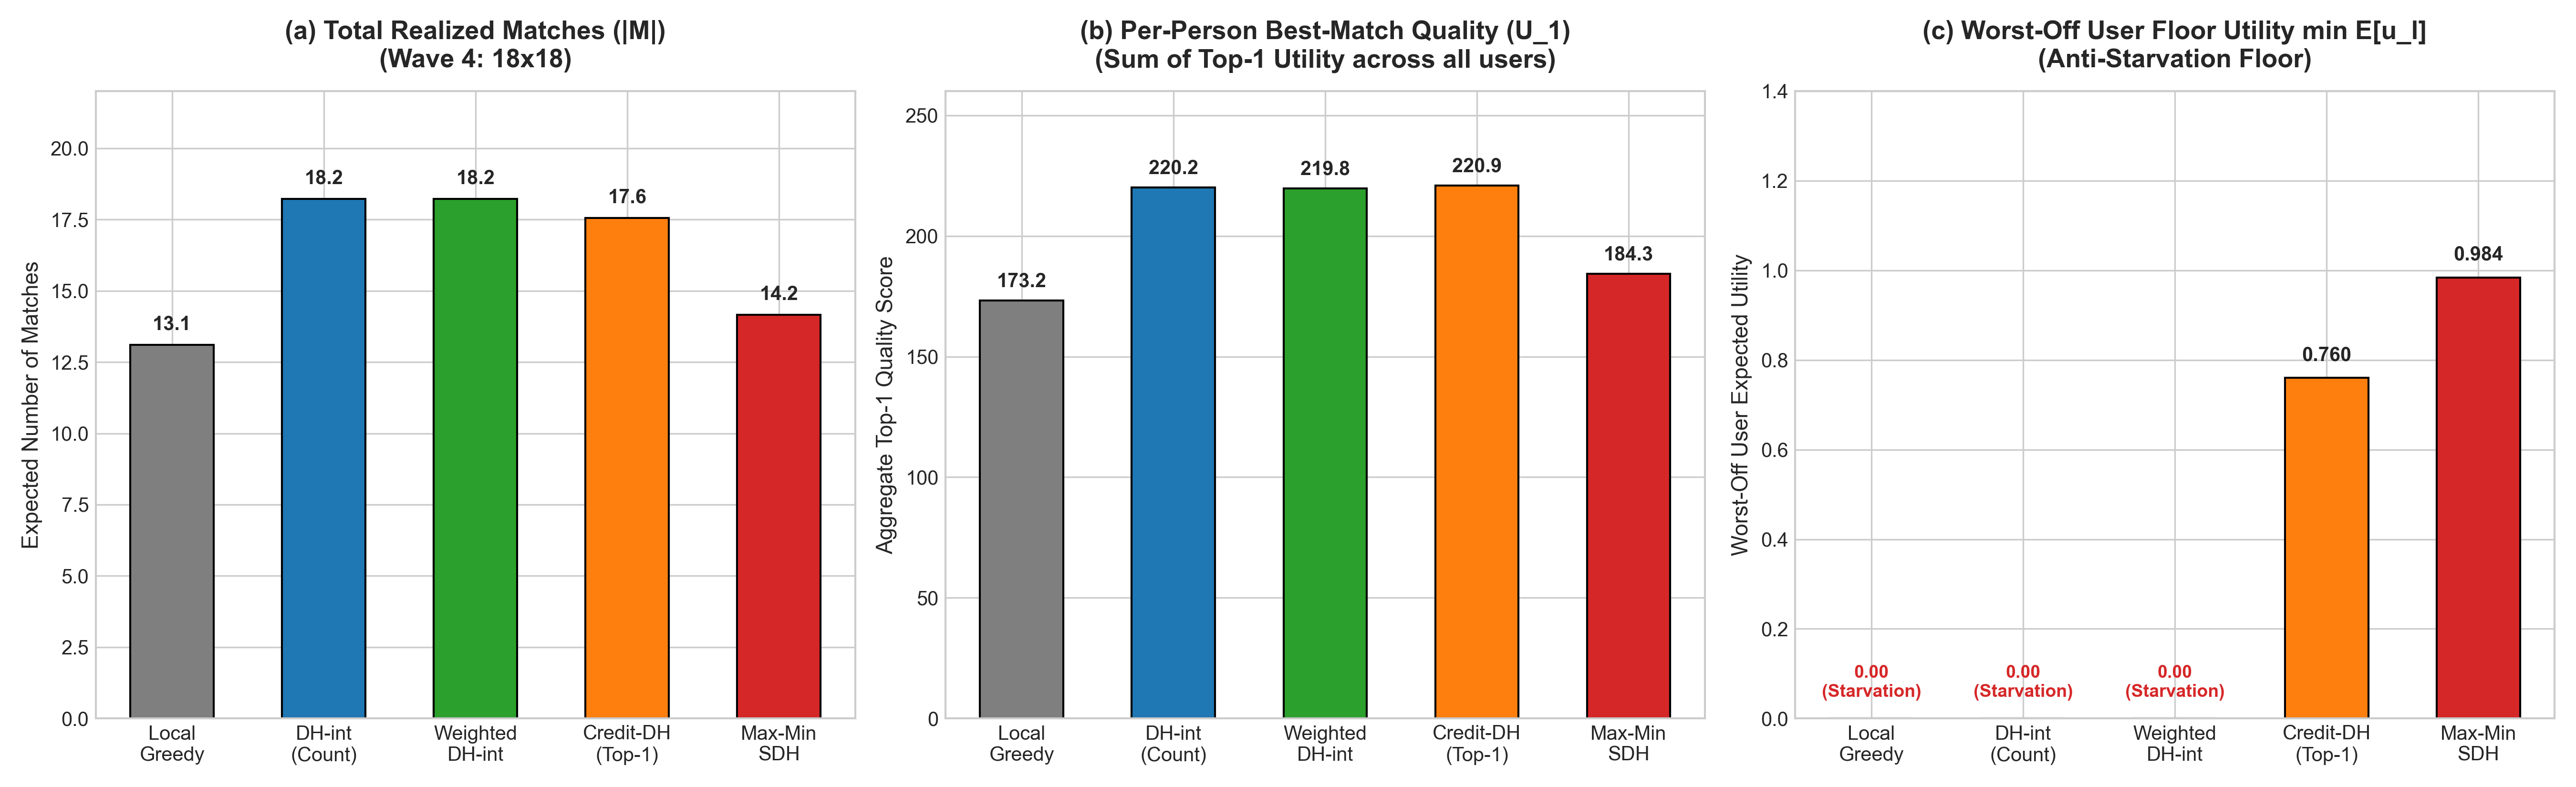
\includegraphics[width=\textwidth]{data/figures/algorithm_comparison_w4.png}
\caption{Comparative performance on Wave 4 ($18\times 18$ market, $K=2$, $500$ trials). (a) DH-int and Credit-DH break market congestion, boosting match volume by $+39\%$. (b) Credit-DH maximizes per-person best-match quality ($U_1$). (c) Max-Min SDH protects the welfare floor, raising the worst-off user's utility from $0.00$ to $0.984$.}
\label{fig:empirical_benchmarks}
\end{figure}

\subsection{Key Empirical Insights}
\begin{enumerate}[leftmargin=2em]
    \item \textbf{DH-int Dominates Local Greedy in Match Volume}:
    On Wave 4, DH-int generates \textbf{$18.22$ matches vs. $13.10$ for Greedy} ($+39.1\%$ increase in successful matches). Local Greedy suffers from heavy congestion: multiple initiators crowd around the same popular candidates, leaving many backlog responses unreciprocated.
    \item \textbf{Credit-DH Wins on Per-Person Best-Match Quality}:
    Credit-DH achieves the highest top-1 quality ($121.52$ on Wave 1, $220.94$ on Wave 4), the highest match participation rate ($75.8\%$), and the lowest Gini inequality ($0.378$). By capping credits at $k=1$, the LP avoids dumping redundant matches on the same popular users and spreads high-quality connections across the entire population.
    \item \textbf{Max-Min SDH Eliminates User Starvation}:
    Under Greedy, DH-int, and Weighted DH-int, the worst-off user's expected utility is \textbf{$0.000$} (disadvantaged or niche users receive zero viable dates). Max-Min SDH raises the welfare floor to \textbf{$1.618$ (Wave 1)} and \textbf{$0.984$ (Wave 4)}, completely eliminating user starvation at the cost of a moderate reduction in total market volume.
\end{enumerate}

\newpage
% =============================================================================
\section{Practical Realities: What Breaks in Real Platforms?}
\label{sec:real_world}
% =============================================================================

If an engineering team at Tinder, Bumble, or Hinge attempted to deploy this exact theoretical pipeline into production tomorrow, where would it break?

\subsection{The Computational Latency Barrier}
* \textbf{Theory}: DH-int, Credit-DH, and SDH solve a Mixed-Integer Program (MIP) across all active users.
* \textbf{Production Reality}: In large metropolitan areas (e.g., London, New York), active user pools exceed $100,000$ individuals. Solving an NP-hard MIP across millions of binary edge variables $x_{\ell\ell'}$ cannot be done in real time. Real-time recommendation feeds must respond within **$30\text{--}50$ milliseconds**.
* \textbf{Engineering Adaptation}: Real platforms decompose matching into a two-stage funnel:
  1. \emph{Candidate Generation}: Fast approximate nearest-neighbor (ANN) search over dense user embeddings.
  2. \emph{Scoring and Reranking}: Passing the top 100 candidates through a lightweight neural ranking model, where the mathematical insights of DH-int (marginal lookahead bonuses) can be applied as scoring terms rather than a global MIP.

\subsection{Backlog Delay vs. User Impatience and Churn}
* \textbf{Theory}: The algorithm deliberately withholds incoming likes in period 1 because the mathematical lookahead proves that holding the like for period 2 maximizes global welfare.
* \textbf{Production Reality}: Users demand instant gratification. If a user receives a like, withholding it for three days leads the user to believe the app is inactive, inducing churn. Platforms like Bumble explicitly enforce a 24-hour expiration rule to force immediacy.

\subsection{Economic Feasibility of LLM Oracles}
* \textbf{Theory}: The LLM oracle evaluates pairs to screen compatibility before display.
* \textbf{Production Reality}: Across $100,000$ users each evaluating $50$ potential candidates, pre-screening requires **$5,000,000$ LLM inferences per cycle**. At current API rates, the cloud computation cost would completely dwarf subscription revenues. LLM screening must be distilled into compact, pre-computed offline vector embeddings.

\subsection{The Business Model Paradox (The Alignment Problem)}
* \textbf{Theory}: The algorithm's objective is to deliver each user their optimal soulmate ($k=1$) as rapidly and efficiently as possible.
* \textbf{Commercial Reality}: Dating platforms operate on recurring subscription models (Tinder Gold, HingeX) and micro-transactions (Boosts, Roses). A platform that instantly matches every user with their lifelong partner in week 1 experiences immediate app deletion and loses customer lifetime value (LTV). Commercial algorithms are designed to maintain \emph{hopeful engagement}, balancing good matches against session retention.

\newpage
% =============================================================================
\section{Lean 4 Formalization Landscape}
\label{sec:lean_landscape}
% =============================================================================

A hallmark of this project is that all theoretical claims have been audited and formalized in **Lean 4** with **Mathlib**, totaling **777 machine-checked theorems** with zero `sorry` placeholders. Table \ref{tab:lean_files} provides a reference mapping between the conceptual topics in this monograph and the corresponding proof files in \texttt{lean/DatingAlgo/}.

\begin{table}[ht]
\centering
\small
\begin{tabular}{@{}llp{8.5cm}@{}}
\toprule
Topic & Primary Lean File & Key Proved Results \\
\midrule
\textbf{Paper Foundations} & \texttt{TwoPeriod.lean} & Lemma C.5, Theorem 4.3 ($(1-1/e)$ approximation for DH-int) \\
& \texttt{Submodularity.lean} & Lemma 4.1 ($f$ monotone submodular), Lemma C.2 \\
& \texttt{CorrelationGap.lean} & Top-$K$ correlation gap from scratch; $c_K \ge 1-1/e$ \\
\midrule
\textbf{Audits \& Repairs} & \texttt{MultiPeriod.lean} & Theorem 5.4 refuted (\texttt{theorem\_5\_4\_counterexample}, ratio 0.50) \\
& \texttt{MultiPeriodDHT.lean} & Theorem 5.3 refuted (\texttt{theorem\_5\_3\_counterexample}, ratio 0.519) \\
& \texttt{MultiPeriodRepair.lean} & Repaired Theorem 5.3 ($\text{DHT-}\tau \ge (1-1/e) \mathrm{OPT}$) \\
\midrule
\textbf{Match Quality} & \texttt{PoissonGap.lean} & Result R1 ($c_K$ Poisson bound), Result R2 (Weighted DH-int) \\
& \texttt{QualityBounds.lean} & Result R3 (Price of counting, $\Theta(1/\rho)$ bound) \\
& \texttt{QualityTopK.lean} & Result R4 ($2k/(K+k)$ upper bound on additive optimization) \\
\midrule
\textbf{Strategic Swiping} & \texttt{TruthfulSwiping.lean} & Theorem 1 (Cost-separability), SDH DSIC truthfulness \\
& \texttt{ScreenedDH.lean} & SDH welfare guarantees ($c_K^2 \mathrm{OPT_{IR}}$), screening bounds \\
& \texttt{PriceOfIR.lean} & Theorem 2 (Price of IR, $k/b$ bound via edge coloring) \\
& \texttt{EdgeColoring.lean} & König's edge-coloring theorem from Hall's Marriage Theorem \\
\bottomrule
\end{tabular}
\caption{The Lean 4 Formalization Landscape (all 777 theorems verified).}
\label{tab:lean_files}
\end{table}

\section{Conclusion}
This monograph has traced the algorithmic and game-theoretic evolution of two-sided matching on modern dating platforms. By transitioning from unweighted match counting to per-person top-$k$ quality, and from passive coin-flipping agents to strategic users with reservation costs, we transform an ad-hoc heuristic into a rigorous, incentive-compatible economic mechanism. While computational latency and business model misalignments present hurdles for commercial deployment, the structural principles established here provide a foundational blueprint for the next generation of intelligent, welfare-maximizing matching markets.

\end{document}
